\documentclass{whutmod}
\usepackage{metalogo}
\usepackage{float}
\usepackage{subfigure} 
\usepackage{url}
\usepackage[style=caspervector,backend=biber,utf8]{biblatex}
\addbibresource{wenxian.bib}
\team{23}	% 组号
\membera{刘子川}
\joba{编程}
\memberb{程宇}
\jobb{建模}
\memberc{陈荣兴}
\jobc{建模}
\hypersetup{
	colorlinks=true,
	linkcolor=black
}

\title{利用对流扩散方程与溯源算法解决嘉陵江水质铊污染问题}
\tihao{3} % 题号

\begin{document}
	
	%\maketitle
	
	\begin{abstract}
本文基于对流扩散方程建立河流一维水质模型,求解出一维河道点源污染浓度变化解析解,估计下游浓度变化趋势,确定重点监测区域和时间。再利用直线解析算法溯源,从而对污染源类型和距离做出合理估计。最后结合嘉陵江铊污染事件的监测数据对模型进行误差分析并检验其合理性。
   ~\\
   
针对问题一, 建立水质监测模型确定重点监测时间和区域。利用对流扩散方程建立河流一维水质模型。经过拉普拉斯变换得到一维污染物浓度随时空变化的解析解。分别根据点污染与面污染的特点得到对应的浓度分布图,并得出重点监测区域和时间。得到的模型符合实际,精度较高。   
~\\

针对问题二,采用直线朔源算法估计污染类型与大致位置。对问题一中的一维污染扩散模型进行线性变换,将问题一中的模型转化成线性模型。利用相关极值法,确定变换后模型中间参数估算污染源大致位置和类型。通过仿真验,对污染浓度数据加入高斯白噪声得到模拟污染数据,进行三次朔源定位测试,得到误差分别为5.28\%、2.34\%和2.12\%。得到模型抗噪能力较强,具有较高可行性。
   ~\\

针对问题三,采集嘉陵江各断面铊元素监测数据结果,统计分析得到铊元素浓度变化趋势。基于各断面处浓度散点数据,利用matlab统计工具箱,拟合出监测点浓度变化曲线并分析特点:从上游到下游总体浓度变化缓和, 污染事件为点源,且污染铊元素距离源头72km处仍具有较高浓度。
   ~\\
   
针对问题四,
首先查阅数据计算出嘉陵江的平均流速1.3647m/s,以及铊化物在江水中的扩散剂系数25.0823m2/s,初始浓度1.52mg/L。基于问题一中建立的污染物浓度时空分布模型,结合问题三中铊元素污染的相关数据,求解出嘉陵江铊污染事件的重点监测区域为下游83.4km,重点监测时间为污染发生后9.42天。基于问题二的直线朔源模型,得到朔源后结果的表示此次污染为点源污染,污染源头在清风峡上游61.6km,与实际结果69.8km相接近。验证了问题一、二中模型的合理性。
   ~\\

本文中所提到的模型优点主要有两点:一、在与污染源头距离较短时预测抗噪能力较强;二、利用更高定位精度和鲁棒性的直线解析法,溯源追踪能力较强。
  
		\keywords{对流扩散方程\quad  直线解析法\quad  溯源算法\quad 拉普拉斯变换\quad }
		
	\end{abstract}
	
	%目录
	\tableofcontents
	\newpage	%换页符
	
	\section{问题重述}
	\subsection{问题背景}

	铊$(thallium)$是一种剧毒物质,广泛存在于自然界的各种媒介中,但丰度均较低,如陆地层中铊的平均含量为$0.49mg/L$,海洋中的平均含量为$0.013mg/L$。铊化物主要通过含铊矿山的开发利用、矿石冶炼中尘埃沉降等途径进入水环境。铊及其盐类是一类环境危害性极强的水体污染物,甚至低浓度的铊都会对生命体产生严重的毒害作用\parencite{liu2019treatment}。
	
	铊盐类化学物会在骨髓、肾脏等器官内蓄积,造成毛发脱落、肌肉萎缩、中枢神经系统损伤等症状。鉴于铊的剧毒性,我国生活饮用水卫生标准中规定了铊的允许含量为$0.1ug/L$。近年来,水体铊污染已呈现加剧的趋势。
	
	于四川广元市发生的嘉陵江铊污染事件, 监测中心站监测嘉陵江入川断面水质异常,西湾水厂水源地水质铊元素超标$4.6$倍。初步判定污染源为川陕界上游输入型、一次性污染团。
	
	当出现水质重金属污染超标时,要尽早快速地诊断出污染类型及污染位置,并切断污染源,减少污染对环境、民众工作生活带来的损失。
	
	\subsection{问题概述}
	
	围绕嘉陵江水体中铊污染事件,依次提出以下问题:
	
	\begin{itemize}
		\item [(1)]
		 给出模型要求出现水体铊元素点源污染或非点源污染时, 能预测分析下游水质中铊元素浓度变化趋势,并估计重点监控区域及时间。
		\item [(2)] 
		根据下游水质检测的数据来估计上游污染类型及污染源位置。
		\item [(3)] 收集铊污染时间相关数据,分析本次铊污染主要特点。
		\item [(4)] 结合问题三的数据,验证问题一二模型结果的合理性。
	\end{itemize}
	
	\section{模型假设}
	\begin{itemize}
		\item [(1)] 假设只考虑污染物在河流中的纵向扩散作用。由于嘉陵江纵向长度远大于江面宽度,可视作不考虑污染物横向的扩散。
		\item [(2)] 
		假设河流中河段均匀、一次性排污和水文条件稳定。为将嘉陵江简化为一维模型计算,可合理假设河流水稳定。
		\item [(3)]
		只考虑干流污染情况.对支流变化不予考虑。由于主要受影响的是嘉陵江主干地区,可忽略污染情况对支流的影响。
		\item [(4)]
		不考虑铊元素及盐产物在水中的衰减系数。由于铊化物属于重金属,且污染天数远小于铊化物分解时间,可不考虑铊污染衰减系数。
		\item [(5)] 为简化模型,假设断面中的污染物浓度是均匀的。
	\end{itemize}
	
	
	\section{符号说明}
	\begin{center}
		\begin{tabular}{cc}
			\hline
			\makebox[0.3\textwidth][c]{符号}	&  \makebox[0.4\textwidth][c]{意义} \\ \hline
			$C_{0}$	    &  污染源初始浓度 \\ \hline
			$C(x,t)$	    &  污染浓度随时空变化 \\ \hline
			$u_{x}$	    &  江河平均纵向流速 \\ \hline
			$E_{x}$  &  铊在江河纵向弥散系数\\ \hline
		$p$   &  面污染物纵向距离\\ \hline
			$K_{c}$	    & 污染物降解系数  \\ \hline
		    $a$	& 污染超标系数 \\ \hline
		     $x$	& 距污染源的一维距离 \\ \hline
		      $t$	& 距污染发生后的时间 \\ \hline
		       $V_{A}$	& 溶液摩尔体积 \\ \hline
		      $M_{B}$	& 江水的摩尔质量 \\ \hline
		     $\mu_{B}$	& 溶剂的粘度 \\ \hline		      
		\end{tabular}
	\end{center}



		%\subsubsection{模型建立与求解}
	
	\section{问题一模型的建立与求解}
	\subsection{问题一描述与分析}
	%\subsubsection{问题一描述与分析}
	针对问题一,假设当出现铊元素的点污染或面污染时,判断下游的重点监控区域和时间。根据对流扩散方程建立污染物浓度关于时间和空间的变化模型,分别根据污染物点源污染与面源污染特点求出起始断面的污染物浓度变化,并且假设零时刻河流下游污染物浓度为零。由此可以得到整个流域的实时污染物浓度变化模型,由此估计出下游污染重点监测区域和时间。

	对流扩散方程是描述流体的非线性方程的线性化模型方程,可以用来描述河流污染中污染物质的分布等物理现象,探索江河突发铊污染事件后污染物在水中动态分布和迁移扩散规律。

	\subsection{模型的建立与求解}
	对于一般河流而言,纵向标度(河长)于横向标度(河宽)之比往往比较大,排入河流的污染物可以假设为在排入水体很短一段距离就可以均匀混合。因此,不考虑混合的距离。大多数河流水质计算可以简化为一维水质模型,即只考虑污染物顺河长方向的污染程度,而不考虑河流河宽(横向)、河深(竖向)的影响。

	根据查阅点源污染资料,在河流的起始断面$x_{0}=0$上,把一质量为$M$的污染物瞬间排放于流速为$u$的河水中,假设污染物即可瞬时与此段面的河水相混合,使得起始断面的初始浓度为$C_{0}$ ,同时刻下游断面的污染物浓度为零\parencite{张永祥2018龙江河镉污染分布及迁移研究},此模型的特征方程可表示为:
	
		\begin{gather}
\frac{\partial c}{\partial t}+u_{x}\frac{\partial c}{\partial x}=E_{x}\frac{\partial^{2} C}{\partial x^{2}}-Kc
\end{gather}
	式中:$E_{x}$为 纵向分散系数,$K_{c}$为污染物的降解系数,
	$\frac{\partial c}{\partial t}$ 浓度随时间的变化率,$\frac{\partial c}{\partial x}$ 浓度随空间的变化率。
	
	且根据点污染的特点得出,起始断面处浓度变化为:
	\begin{gather*}
	C(0,t)=C_{0}\delta (t)\\
	 C(x,0)=0(x>0)
	\end{gather*}
	式中,污染物浓度$C(0,0)=C_{0}$,$E_{x}$为河水的纵向弥散系数,$K$为污染物的降解系数,由于重金属的降解速率较慢,即可视为$K=0$,表达式可简化为:
		\begin{gather*}
	 \frac{\partial c}{\partial t}+u_{x}\frac{\partial c}{\partial x}=E_{x}\frac{\partial^{2} C}{\partial x^{2}}
	\end{gather*}
	对方程进行拉普拉斯变换求解\parencite{张永祥2018龙江河镉污染分布及迁移研究},得一维河道点源污染浓度随时间和距离变化的动态解如下:
			\begin{gather}
	c(x,t)=\frac{u_{x}C_{0}}{2\sqrt{\pi E_{x}t}}exp[-\frac{(x-u_{x}t)^{2}}{4E_{x}t}]
	\end{gather}
	
	查阅资料可得\parencite{geng2019novel},面源污染是由于雨水的冲刷和渗透作用直接造成的,可将模型改进为初始面源污染距离$x_{0}$的一段积分\parencite{xie2019intra}:
			\begin{gather}
c(x,t)=\int_{x}^{x+x_{0}}\frac{u_{x}C_{0}}{2\sqrt{\pi E_{x}t}}exp[-\frac{(p-u_{x}t)^{2}}{4E_{x}t}]dp
	\end{gather}
	
	由上式可得到一维河道污染物浓度分布随时间推移过程图~\ref{llllll}~:
			
	\begin{figure}[H]
		\centering
		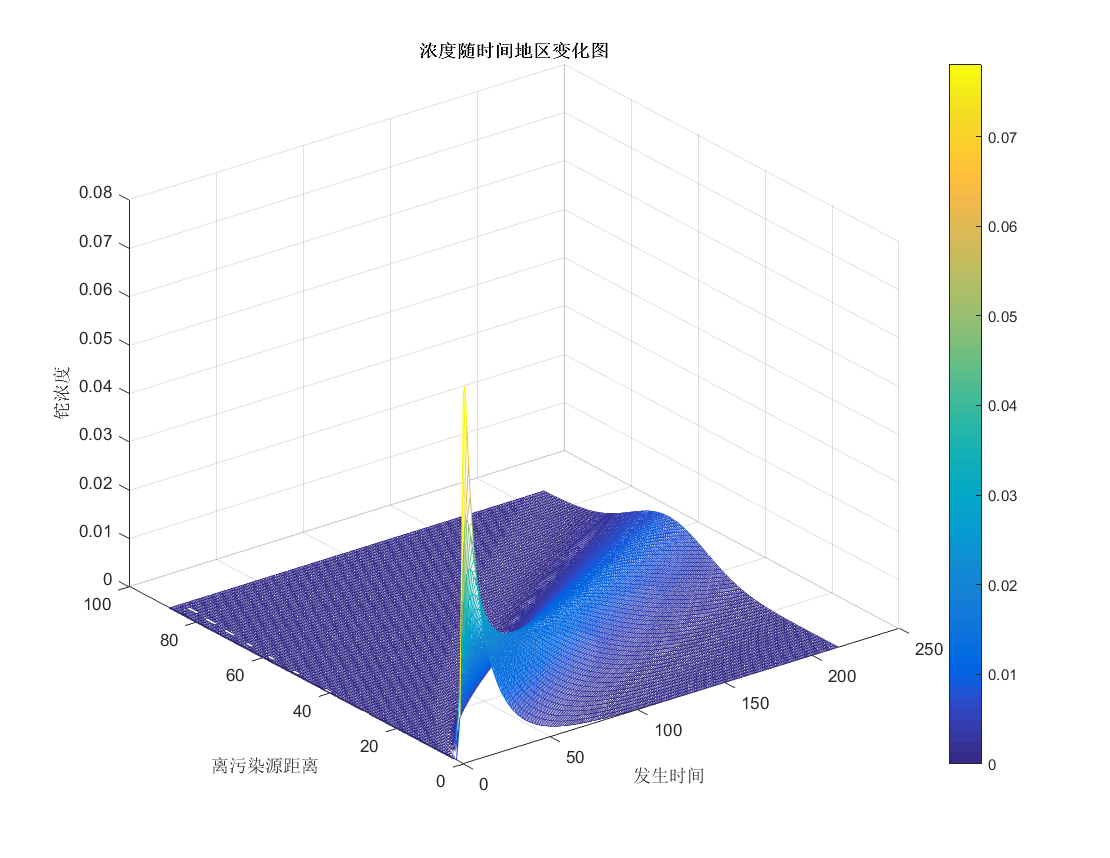
\includegraphics[width=\textwidth]{figures/matlab.png}
		\caption{浓度分布随时间推移过程图}\label{llllll}
	\end{figure}
	
	为方便分析,分别取瞬时点污染源扩散12h,24h,48h,72h,96h时,
	对污染物浓度分布情况图进行对比分析,具体浓度分布如图~\ref{wrw}~所示:
		\begin{figure}[H]
	\centering
	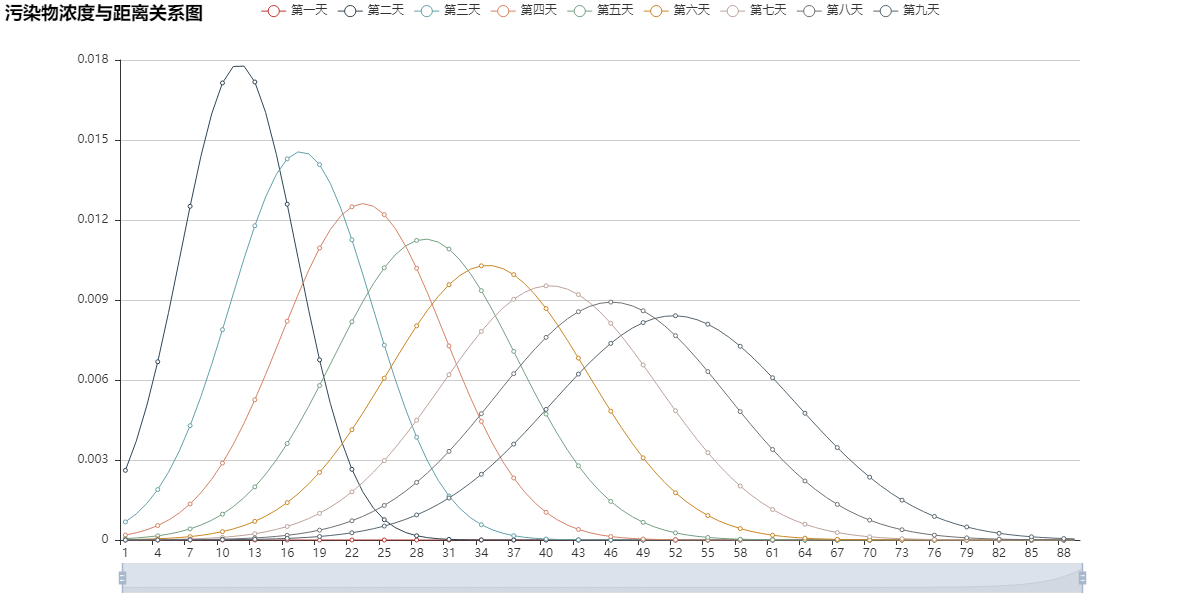
\includegraphics[width=\textwidth]{figures/wrw.png}
	\caption{污染物浓度与距离关系图}\label{wrw}
	\end{figure}

	由图可知一维河道点源污染的扩散峰值随着时间的增加向河流速度方向推移,不妨令平均移动速度为$25m/min$时,严重污染带(污染物浓度>$
	aC_{0}$)随着时间的增加先增大后减小。     
	
	当污染浓度$C>aC_{0}$时得到所需监控时空区域图如图~\ref{ndfb}~所示:
		\begin{figure}[H]
	\centering
	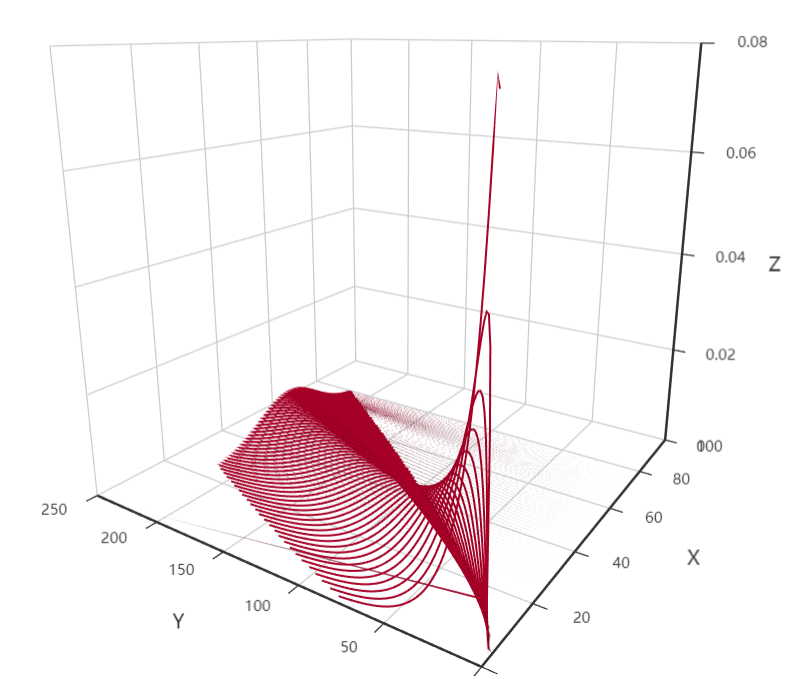
\includegraphics[width=\textwidth]{figures/ndfb.png}
	\caption{监控时空区域图}\label{ndfb}
\end{figure}
	
	即当污染发生后,重点监测区域及其对应时间如图~\ref{hblq}~所示:
			\begin{figure}[H]
		\centering
		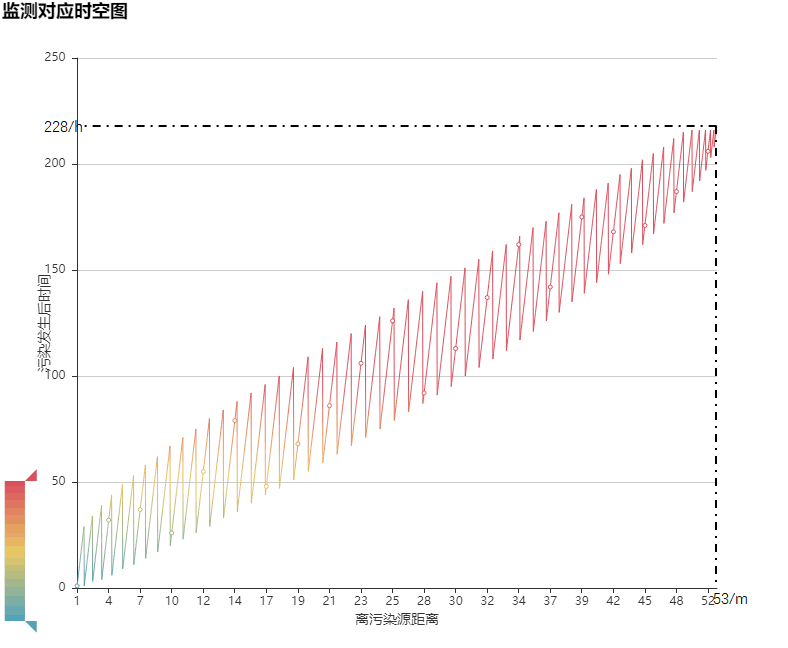
\includegraphics[width=.9\textwidth]{figures/hblj.png}
		\caption{监测区域及其对应时间}\label{hblq}
	\end{figure}
	由图~\ref{hblq}~所示,根据算例所给参数表明,当污染发生后,其重点监控的区域是从0<x<53km;重点监控的时间是从0<t<228h。

	
	\subsection{结果分析}
	\begin{itemize}
		\item [(1)] 当时间t和空间距离x趋于无穷大时,由模型算得污染物浓度趋近于0,符合实际情况。
		\item [(2)] 
	模型所解出的重点监测区域捕捉了严重污染带的时空分布特点,并且完全包含了严重污染带的时间、空间范围。

	\end{itemize}

	\section{问题二模型的建立与求解}
	\subsection{问题二描述和分析}
	针对问题二,要求当下游监测到铊元素污染超标时对污染源的类型进行快速判断以及对位置进行定位,利用直线解析算法对问题一中一维污染扩散模型进行适当变形,根据相关极值法原理,推导出了中间参数的计算公式,从而将非线性问题转化为线性问题,通过中间参数和直线常数的求解,可以得到五个参数值,即$M$、$E_{x}$、$u_{x}$、$x_{0}$和$t_{0}$。问题要求对污染源位置进行判断,即通过该模型求出$x_{0}$即可,其流程图如图~\ref{lct}~所示:
			\begin{figure}[H]
	\centering
	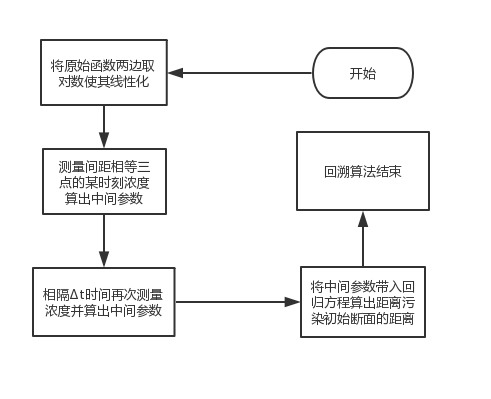
\includegraphics[width=.8\textwidth]{figures/lct.png}
	\caption{算法流程图}\label{lct}
	\end{figure}
	\subsection{模型建立与求解}
	\subsubsection{模型的建立}
	将初始污染发生地点设为$x_{0}$,初始地点设为$t_{0}$,则可修改问题一模型为:
	\begin{gather}
	c(x,t)=\frac{u_{x}C_{0}}{2\sqrt{\pi E_{x}(t-t_{0})}}exp[-\frac{[(x-x_{0})-u_{x}(t-t_{0})]^{2}}{4E_{x}t}]
	\end{gather}
	令观察时刻为零时刻,即$t=0$,得到:
	\begin{gather*}
		c(x,t)=\frac{u_{x}C_{0}}{\sqrt{4\pi E_{x}(t-t_{0})}}exp[-\frac{[(x-x_{0})+u_{x}t_{0}]^{2}}{4E_{x}(-t_{0})}]
	\end{gather*}
	
	对上式两侧取对数,并做参数替换得到一次函数:
	\begin{gather}
	Y=m_{x}X+b_{x}\label{yyy}
	\end{gather}
	其中:
	\begin{gather*}
		\left\{\begin{matrix}
			Y=lnc	\\
		m_{x}=\frac{1}{4E_{x}t_{0}} \\
		X=(x-x_{m})^{2} \\
		x_{m}=(x_{0}-u_{x}t_{0}) \\
		b_{x}=\sqrt{\frac{-m_{x}}{\pi}}ln(u_{x}C_{0})\\
		\end{matrix}\right.
	\end{gather*}
	
	由式~\ref{yyy}~可知,因变量与Y自变量X呈线性关系,斜率和纵截距分别为$m_{x}$和$b_{x}$。因变量$Y$可通过检测对应节点的污染物浓度值$c$求出,自变量$X$因包含了观测点的位置坐标$x$和中间参数$ x_{m}$而无法确定$X$的各点坐标,因次首先要确定中间参数$ x_{m}$。可以通过求解$X$、$Y$的相关系数\parencite{沈凤文2016点源污染的移动式检测定位及应用}即:
	
	\begin{gather*}
		R_{Y,X}=\frac{\sum_{i=1}^{n}(X_{i}-\overset{-}{X})(Y_{i}-\overset{-}{Y})}{\sqrt{\sum_{i=1}^{n}(X_{i}-\overset{-}{X})^{2}\cdot \sum_{i=1}^{n}(Y_{i}-\overset{-}{Y})^{2}}}
	\end{gather*}
	式中$\overset{-}{X}=\frac{1}{n}\sum_{i=1}^{n}X_{i},
	\overset{-}{Y}=\frac{1}{n}\sum_{i=1}^{n}Y_{i}
	$,对相关系数对$x_{m}$求偏导数,使其达到极值0,即$\frac{\partial(R_{X,Y}) }{\partial x_{m}}=0$即可得到中间参数$x_{m}$的计算公式为:
		\begin{gather}
x_{m}=\frac{d_{x}f_{x}-2a_{x}g_{x}}{2f_{x}e_{x}-d_{x}f_{x}}\label{2.6}
	\end{gather}
	其中:
		\begin{gather*}
	\left\{\begin{matrix}
a_{x}=\overline {x^{4}}-(\overline {x^{2}})^{2}	\\
	d_{x}=4\overline {x^{3}}-4\overline {x}\cdot\overline {x^{2}}\\
	e_{x}=4\overline{x^{2}}-4(\overline{x})^{2} \\
	f_{x}=\overline{x^{2}\cdot Y}-\overline{x^{2}}\cdot \overline{Y}\\
	g_{x}=2\overline{xY}-2\overline{x}\cdot \overline{Y}\\
	\end{matrix}\right.
	\end{gather*}
	求得中间参数$x_{m}$后,可以通过式~\ref{2.6}~得到一系列$X_{i}$的值,利用式~\ref{yyy}~计算相应的$Y_{i}$的值,即可通过线性回归法算出相应的斜率$m_{x}$和$b_{x}$。同理,测量计算经过$\Delta t$时刻后的上述参数,并通过计算得到另一组 ${x_{m}}'$、${m_{x}}'$、${b_{x}}'$。
	
	此时,可以通过以上获得的数据计算一维河道点源污染随流扩散模型的各个参数,计算公式如下:
			\begin{gather}
	\left\{\begin{matrix}
	 u_{x}=\frac{{x_{m}}'-x_{m}}{\Delta t}	\\
	t_{0}=\frac{{x_{m}}'\Delta t}{{x_{m}}'-m_{x}}\\
	x_{o}=x_{m}+u_{x}t_{0} \\
	E_{x}=\frac{1}{4t_{0}m_{x}}\\
	C_{0}=\sqrt{\frac{\pi}{-m_{x}}}exp(b_{x})\\
	\end{matrix}\right.\label{9999}
	\end{gather}
	式中,$u_{x}$为河流流速,$t_{0}$为初始排放污染物时间,$x_{0}$为污染源距离观测点距离,$E_{x}$为污染物纵向扩散系数,$C_{0}$为起始断面零时刻污染物浓度。此时一维河道污染随流扩散模型的各项参数值均可求得,河道污染朔源定位过程结束。
	
			\begin{figure}[H]
		\centering
		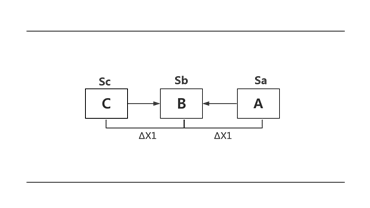
\includegraphics[width=\textwidth]{figures/wrydw.png}
		\caption{污染源定位模拟图}\label{wrydw}
	\end{figure}

由于结合水质检测系统进行定位污染源,污染源定位模型图如上图~\ref{wrydw}~所示,污染源具体定位步骤如下:
		\begin{itemize}
	\item [(1)] A为水质主监测点,B、C分别为副监测点,它们可同时测量污染物浓度参数,
	相隔间距均为$\Delta x_{1}$采样t时刻和$t+\Delta t$时刻三个节点的污染物浓度值进行测量。
	\item [(2)] 
设$S_{a1}$的位置为0,则$S_{b1},S_{c1}$的位置分别为$\Delta x_{1}$和$2\Delta x_{1}$,通过带入直线解析算法推导并计算污染物排放时间$-t$和地点$-x_{0}$。
	\item [(3)]一维河道瞬时污染朔源结束。
\end{itemize}

\subsubsection{朔源仿真算例}

通过直线解析算法的朔源定位流程,将污染物浓度$c_{0}$加入1\%的高斯白噪声作为采样值进行储存。选取扩散后$22h$、$30h$、$38h$时,$900m$、$1200m$、$1500m$左右的范围进行测试,每组包括6个污染物浓度测试值,测量时间为$1h$,测量范围为$300m$,满足可检测的污染物浓度范围带。通过直线解析算法进行一维河道瞬时污染源朔源定位测试,其中$\Delta x_{1}$为$100m$,其测量值如表~\ref{biao}~所示。
	\begin{table}[H]
	\caption{测量值采样点}\label{biao} \centering
	\begin{tabular}{cccc}
		\toprule[1.5pt]
		序号 &采样点设定位置/m&  时间/h & 测得浓度值/\%$C_{0}$ \\
		\midrule[1pt]
		1	& Sa=900 &22 &0.015602172\\
		2	& Sb=800 & 22 &0.019912537\\
		3	& Sc=700 &22 &0.023559553\\
		4	& Sa=900 &23 &0.016619613\\
		5	& Sb=800 &23 &0.020625445\\
		6	& Sc=700 &23&0.023807574\\
		7	& Sa=1200 &30 &0.011899716\\
		8	& Sb=1100 &30 &0.015110705\\
		9	& Sc=1000 &30 &0.018151201\\
		10	& Sa=1200 &31 &0.012694285\\
		11	& Sb=1100 &31 &0.015790862\\
		12	& Sc=1000 &31 &0.018614625\\
		13	& Sa=1500 &38 &0.009394361\\
		14	& Sb=1400 &38 &0.011894481\\
		15	& Sc=1300 &38 &0.014413709\\
		16	& Sa=1500 &39 &0.010030596\\
		17	& Sb=1400 &39 &0.01249462\\
		18	& Sc=1300 &39 &0.01491282\\
		\bottomrule[1.5pt]
	\end{tabular}
\end{table}

通过上述采集数据可得到两个观测时刻的位置和浓度测量数据经过计算得到中间计算值如表~\ref{biao2}~所示。
	\begin{table}[H]
	\caption{溯源结果}\label{biao2} \centering
	\begin{tabular}{cccccccccc}
		\toprule[1.5pt]
		$X_{m}$& $b_{x}$ & $m_{x}$ &${X_{m}}'$ & ${b_{x}}'$&${m_{x}}'$&$x_{0}$/m&实际距离/m& 误差\\
		\midrule[1pt]
		812.65 &-0.00000253 &5.44&1186.89&-0.00000227&5.34&946&900&5.27\%\\
		1374.46& -0.00000255 &5.56&1563.11&-0.00000229&5.45&1171.93&1200&2.34\%\\
		1586.69 &-0.00000257 &5.63&1782.85&-0.0000023&5.52&1526.71&1500&2.12\%\\
		\bottomrule[1.5pt]
	\end{tabular}
\end{table}

由表~\ref{biao2}~所得三次朔源定位位置值,通过式~\ref{9999}~
可得河水流速$u=1.44km/h, (0.4m/s)$,排放时间t1=-21.6h、t2=-29.1h、t3=-36.8h,即瞬时点污染投放的时间为21.6h、29.1h、36.8h之前。

\subsubsection{模拟验证与分析}
 从上述的计算过程中可以分析得到,对朔源算法的主要影响因素为浓度测量噪声和采样时间间隔,通过$Matlab$工具箱针对一维河道污染扩散模型产生模拟数据,对直线解析算法进行一维点源污染定位仿真。

 浓度测量噪声,在模拟背景中,将测量浓度中分别加入1\%、5\%,8\%,10\%的高斯白噪声进行朔源分析,得到定位结果如表~\ref{gsbz}~所示。
		\begin{table}[H]
		\caption{浓度测量噪声对溯源算法的影响}\label{gsbz} \centering
		\begin{tabular}{ccccc}
			\toprule[1.5pt]
			浓度噪声&距离真实值/m&时间真实值/h&距离定位值/m&污染源排放时间反演值/min \\
			\midrule[1pt]
			1\% &1500&38&1475.3&37.3\\
			5\%&1500 &38&1413&36.4\\
			8\% &1500&38&1386&35.8\\
			10\% &1500&38&1664.2&45.5\\
			\bottomrule[1.5pt]
		\end{tabular}
	\end{table}
	由表~\ref{gsbz}~可知,当浓度测量噪声的增加,溯源算法的误差随之增大,但溯源精度都控制在10\%左右,具有较强的可行性。则溯源测量误差小于10\%的前提下,可判断污染源是点源污染;否则可考虑为面源污染。


	\section{问题三模型的建立与求解}
	
	
	\subsection{问题描述}

根据事故后各断面的铊元素浓度监测结果,各监测断面铊元素的浓度随时间的变化而不断的发生变化。查阅相关数据后,统计分析得到5月6日2时至5月11日12时的各监测断面铊元素浓度变化曲线图,如图~\ref{tu}~所示:
				\begin{figure}[H]
		\centering
		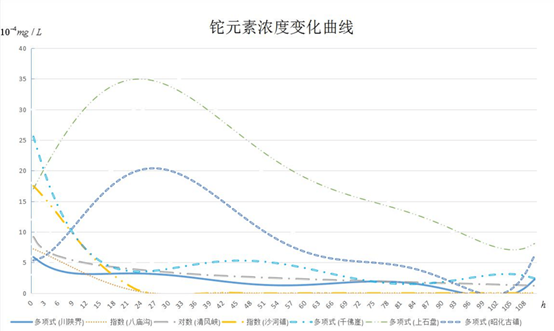
\includegraphics[width=.8\textwidth]{figures/tu.png}
		\caption{各断面铊元素浓度变化图}\label{tu}
	\end{figure}
\subsection{特点分析}
基于各处监测断面处的铊元素散点数据,使用matlab统计工具箱对流域中铊元素浓度数据进行回归分析,绘制出波动性较小,结果更符合预测性的拟合曲线来对铊元素污染特征进行分析,如图~\ref{tu2}~所示,其中浓度单位$10^{-4}mg/L$。
	\begin{figure} [H]
	\centering 
	\subfigure[川峡界流域]{% 
		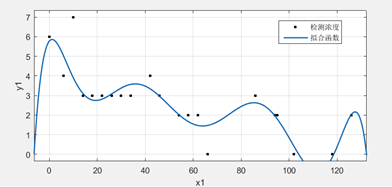
\includegraphics[width=7.5cm]{figures/1.png}}
	\quad
	\subfigure[沙河镇流域]{% 
		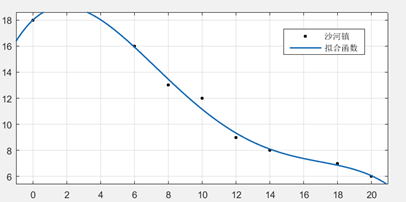
\includegraphics[width=7.5cm]{figures/2.png}}

\end{figure}

\addtocounter{figure}{-1}       %先欺骗LaTeX图形计数器
\begin{figure} [H]
	\addtocounter{figure}{1}      %再告诉LaTeX图形计数器真相
	\centering 
		\quad
	\subfigure[张王乡流域]{
		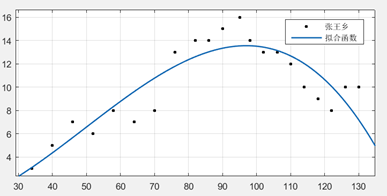
\includegraphics[width=6.5cm]{figures/3.png}
	}
	\quad
	\subfigure[清风峡流域]{
		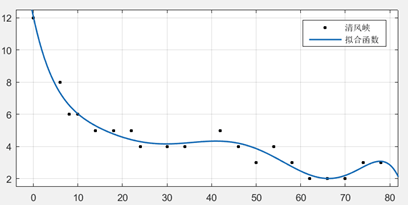
\includegraphics[width=6.5cm]{figures/4.png}
	}
	\quad
	\subfigure[千佛崖流域]{
		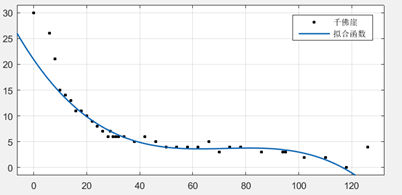
\includegraphics[width=6.5cm]{figures/5.png}
	}
	\quad
	\subfigure[江口镇流域]{
		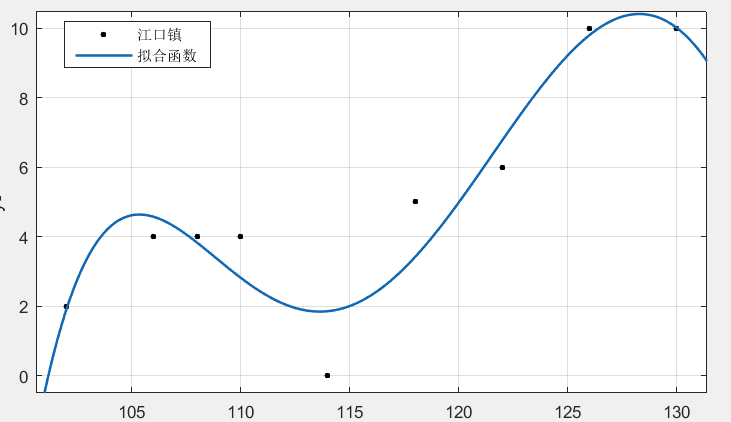
\includegraphics[width=6.5cm]{figures/6.png}
	}

	\caption{各地区拟合结果图}\label{tu2}
\end{figure}

从图~\ref{tu2}~中可以看出,随着时间的累计和携带铊元素流域的不断扩张,铊元素化合物与整个水体完成混合,监测到的浓度从上游到下游逐渐减小,所需重点监控的地区范围开始缩小,监控时长也在缩短。铊元素的浓度变化较平缓,具有一定的可研究型和变化趋势可预测性。图中当各流域监测点出现铊浓度大于0.0001mg/L时,即可确定重点监测区域和时间段。

各地区监测到的铊元素浓度一直发生着显著的变化,推测出此次污染事件为点源污染。若为面源污染,污染浓度变化率比点源发出的污染浓度变化率小。面源污染在刚开始的污染传播断面中浓度就已均匀分布,而铊元素若为点源污染源,随流域扩张浓度不断发生大范围变化。

此次事件中的铊浓度在上石盘和昭化古镇流域达到较高值,参考相关地理信 息和嘉陵江临江距离,可得出铊污染在距离源头$72km$处左右仍具有较高的污染值,有 关部门需要对此地区采取强于其他流域地区的铊吸附沉降措施。

	\section{问题四模型的建立与求解}
	\subsection{问题描述与分析}
	针对问题四,首先根据问题三中本次铊元素污染的相关数据,基于问题一中所建立的污染物浓度的时空分布模型,进行相关分析。将问题三中的实际数据带入问题一的模型中,在已知各监测站之间的距离、水流速度的条件下,得出本次陵江铊污染发生后所应该监测的重点区域以及相应时间。然后利用模型二,求解出本次陵江铊污染的污染源大致位置。最后将模型的距离与所查实际做对比,由此验证模型合理性。
		 \subsection{预备工作}
	\subsubsection{估算嘉陵江平均流速}
	河流断面的平均流速计算,选取嘉陵江最大流速和最小流速作为输入数据,考虑河流上游河床陡峭和中下游河床平缓,引入河流上下游高度,对最大最小流速进行加权计算,得平均流速的估计值,其公式如下\parencite{ahn2019uncertainty}:
	
	\begin{gather}
	u_{x}=V_{max}p_{1}+V_{min}p_{2}
	\end{gather}
	
	
	上游长度为$357km$,中下游长度为$988km$,权数$p1=0.2654,p2=0.7346$,查阅资料\parencite{邓朝华2017浅谈长江航道表面流速流向的数据采集}可得嘉陵江全年中$ V_{max} =4.09m/s$,$ V_{min}=0.38m/s$得平均流速得估计值为 $u_{x}=1.3647m/s$。 

	\subsubsection{铊化物在江水中的扩散系数}
	铊元素及其盐产物在江水中的含量较低,可以假设江水为低浓度的非电解质溶液,铊元素在江水中的扩散系数  $E_{x}$可由$Wilke-Chang$公式\parencite{miyabe2011estimation}计算:
	\begin{gather}
	E_{x}=\frac{7.4\times 10^{-15}T(\phi _{B}M_{B})^{0.5}}{\mu _{B}V{_{A}}^{0.6}}
	\end{gather}
	
	式中:A表示铊元素及其盐产物,B为江水,$V_{A}$表示溶质摩尔体积$cm^{3}/mol$, 
	$\phi_{B}$为江水的缔合参数,T为江水的温度(设定为25℃) ,
	$M_{B}$江水的摩尔质量,
	$\mu_{B}$为溶剂B的粘度。求得铊化物在水中的扩散系数为$25.0823m^{2}/s$。
	\subsection{模型的建立与求解}
对于问题一的解答:由上述相关计算并查阅资料后,得到流速$u_{x}=1.3647m/s$、 $E_{x}=25.0823m^{2}/s$ 初始污染浓度$C_{0}=1.52mg/L$,超标区浓度大于$0.0001mg/L$,即令$C>0.0001mg/L$, 得到时空区域图如图~\ref{skfbt}~所示:
\begin{figure}[H]
	\centering
	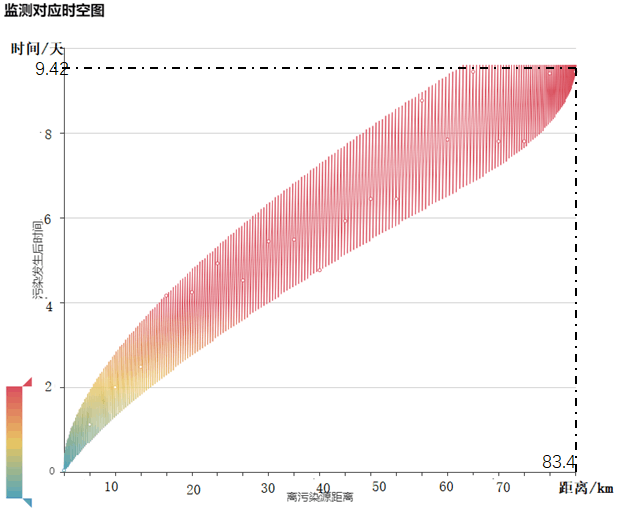
\includegraphics[width=.8\textwidth]{figures/zaojiatu.png}
	\caption{从污染源开始监测范围}\label{skfbt}
\end{figure}
得到污染事故发生后重点监测区域为下游83.4km,后重点监测时间段为9.42天。与实际在广元市超标距离与时间相符,验证了问题一的合理性。
~\\

对于问题二的解答:取下游等距离三点分别为清风峡、沙河镇、千佛崖,取清风峡坐标值为0,得到表~\ref{zzz}:
	\begin{table}[H]
	\caption{铊污染事件溯源结果}\label{zzz} \centering
	\begin{tabular}{cccccccccc}
		\toprule[1.5pt]
		$C_{c}$& $C_{b}$ & $C_{a}$ &${C_{c}}'$ & ${C_{b}}'$&${C_{a}}'$&$x_{0}$/km&实际距离/km& 误差\\
		\midrule[1pt]
		0.00068&0.00013 &0.0020&0.00065&0.00012&0.00011&-61.6&-69.8&5.56\%\\
		0.00012& 0.00182 &0.00301&0.00081&0.00167&0.00262&-53.6&-69.8&7.86\%\\
		\bottomrule[1.5pt]
	\end{tabular}
\end{table}
由表~\ref{zzz}~可得出该污染为点源污染,并算出监测点距离污染源头在61.6km,与实际距离69.8km相接近,误差最小仅为5.56\%,验证了问题二的合理性。


	\section{模型的评价}
	\subsection{模型的优点}
	本文借鉴传统定位方法进行改进,结合水质检测系统研究一维河道瞬时点源污染,利用具有更高定位精度和鲁棒性的直线解析法,在污染发生后,短距离内朔源追踪的精度较高强。
	
	\subsection{模型的缺点}
模型仅考虑了污染物的纵向扩散作用,并未考虑在水中的横向扩散作用及垂直扩散作用,不具有二维浓度变化的特性。在判断面源污染时,仅根据误差分析进行判断,未进行定量分析。


	\subsection{模型的改进与展望}
本文建立的一维水质经考虑了污染物的纵向扩散作用,适用于污染物均匀混合的断面下游。在此基础之上可以对一维污染物浓度变化模型加以改进建立二维污染物浓度变化模型,不仅考虑污染物纵向扩散作用还考虑污染物横向扩散作用,由此预测在污染物与河水均匀混合断面前的污染物浓度变化。
	\newpage	%换页符
	%%参考文献
	%\begin{thebibliography}{9}%宽度9
	% \setlength{\itemsep}{-2mm}
	
	\printbibliography[title = {参考文献}]	%使用国标参考文献添加方式
	
	% \bibitem{bib:one} 
	% 韩中庚. 数学建模方法及其应用[M]. 高等教育出版社, 2005.
	% \bibitem{bib:two}
	% 韩中庚. 数学建模方法及其应用[M]. 高等教育出版社, 2005.
	% \bibitem{bib:two}
	% 韩中庚. 数学建模方法及其应用[M]. 高等教育出版社, 2005.
	% 
	% \nocite{*}		%排版未引用的参考文献
	% \bibliography{文献数据库}	%不同书库用数据分割
	%
	%\end{thebibliography}
	
	\newpage
	%附录
	\appendix %%附录
\section{代码}
\subsection{数据预处理--matlab源代码}
\begin{lstlisting}[language=matlab]
x=linspace(0,20000); y1=exp(-0.00075*x); y2=exp(-0.00079*x); y3=exp(-0.00086*x); y4=exp(-0.00090*x); y5=exp(-0.00118*x); y6=exp(-0.00105*x); y7=exp(-0.00111*x); y8=exp(-0.00117*x); y9=exp(-0.00118*x);
plot(x,y1); hold on plot(x,y2); plot(x,y3) 
plot(x,y4)
plot(x,y5)
plot(x,y6)
plot(x,y7)
plot(x,y8)
plot(x,y9)
scdxzzhold on
line([0,10000],[6.5785e-5,6.5785e-5])
[x,y] = ginput(1)

\end{lstlisting}
\subsection{偏微分方程公式求解--python源代码}
\begin{lstlisting}[language=python]
import pandas as pd
import numpy as np
import csv
import math
import matplotlib.pyplot as plt
from mpl_toolkits.mplot3d import Axes3D
from pyecharts import Scatter3D
import pyecharts




#总路程8900m
DIS = 8900
#间隔100m
X_interval = 100
#总时间240h
T_ALL = 24*9
#时间间隔1h
T_interval = 1
#初始浓度
C0 = 1
#流速
u = (0.4*60)
# u = 1.3647
#离散速度
E = (50*60)
# E = 0.01
if __name__ == "__main__":
# print("程宇牛逼!!!")
#当前污染浓度
c = 0
#离污染源距离
x = 1
#污染后时间
t = 1
# ax = plt.figure().add_subplot(111)

cities=[]
highs1=[]
highs2=[]
highs3=[]
highs4=[]
highs5=[]
highs6=[]
highs7=[]
highs8=[]
highs9=[]
while x <= (DIS/X_interval):
while t <= (T_ALL/T_interval*9):
X = x*X_interval
T = t*T_interval
c = ((u*C0)/(2*np.sqrt(np.pi*E*T)))*np.e**((-(X-u*T)**2)/(4*E*T))
print(c)
t += 1
highs1.append(c)
t=1
while t <= (T_ALL/(T_interval*9/2)):
X = x*X_interval
T = t*T_interval
c = ((u*C0)/(2*np.sqrt(np.pi*E*T)))*np.e**((-(X-u*T)**2)/(4*E*T))
print(c)
t += 1
highs2.append(c)
t = 1
while t <= (T_ALL/(T_interval*9/3)):
X = x*X_interval
T = t*T_interval
c = ((u*C0)/(2*np.sqrt(np.pi*E*T)))*np.e**((-(X-u*T)**2)/(4*E*T))
print(c)
t += 1
highs3.append(c)
t = 1
while t <= (T_ALL/(T_interval*9/4)):
X = x*X_interval
T = t*T_interval
c = ((u*C0)/(2*np.sqrt(np.pi*E*T)))*np.e**((-(X-u*T)**2)/(4*E*T))
print(c)
t += 1
highs4.append(c)
t = 1
while t <= (T_ALL/(T_interval*9/5)):
X = x*X_interval
T = t*T_interval
c = ((u*C0)/(2*np.sqrt(np.pi*E*T)))*np.e**((-(X-u*T)**2)/(4*E*T))
print(c)
t += 1
highs5.append(c)
t = 1
while t <= (T_ALL/(T_interval*9/6)):
X = x*X_interval
T = t*T_interval
c = ((u*C0)/(2*np.sqrt(np.pi*E*T)))*np.e**((-(X-u*T)**2)/(4*E*T))
print(c)
t += 1
highs6.append(c)
t = 1

while t <= (T_ALL/(T_interval*9/7)):
X = x*X_interval
T = t*T_interval
c = ((u*C0)/(2*np.sqrt(np.pi*E*T)))*np.e**((-(X-u*T)**2)/(4*E*T))
print(c)
t += 1
highs7.append(c)
t = 1
while t <= (T_ALL/(T_interval*9/8)):
X = x*X_interval
T = t*T_interval
c = ((u*C0)/(2*np.sqrt(np.pi*E*T)))*np.e**((-(X-u*T)**2)/(4*E*T))
print(c)
t += 1
highs8.append(c)
t = 1
while t <= (T_ALL/T_interval):
X = x*X_interval
T = t*T_interval
c = ((u*C0)/(2*np.sqrt(np.pi*E*T)))*np.e**((-(X-u*T)**2)/(4*E*T))
print(c)
t += 1
highs9.append(c)
t = 1

cities.append(x)
x+=1

print(str(len(cities))+"。。。。"+str(len(highs1)))
line = pyecharts.Line("污染物浓度与距离关系图", width=1200, height=600)
line.add("第一天", cities, highs1,is_symbol_show=True, is_datazoom_show=True)
line.add("第二天", cities, highs2,is_symbol_show=True, is_datazoom_show=True)
line.add("第三天", cities, highs3,is_symbol_show=True, is_datazoom_show=True)
line.add("第四天", cities, highs4,is_symbol_show=True, is_datazoom_show=True)
line.add("第五天", cities, highs5,is_symbol_show=True, is_datazoom_show=True)
line.add("第六天", cities, highs6,is_symbol_show=True, is_datazoom_show=True)
line.add("第七天", cities, highs7,is_symbol_show=True, is_datazoom_show=True)
line.add("第八天", cities, highs8,is_symbol_show=True, is_datazoom_show=True)
line.add("第九天", cities, highs9,is_symbol_show=True,is_datazoom_show=True)
line.show_config()
line.render('demo.html')

# # 显示图像
# plt.show()

# ax = plt.figure().add_subplot(111, projection='3d')
#
# fig = plt.figure()
# ax = fig.add_subplot(111, projection='3d')
#
# if __name__ == "__main__":
#
#     c = (1-2*E*T_interval/(X_interval**2))*0+T_interval*(E/(X_interval**2)-u/(2*X_interval))*0+T_interval*(E/(X_interval**2)+u/(2*X_interval))
#     print(c)
\end{lstlisting}
\subsection{数据拟合分析--matlab源代码}
\begin{lstlisting}[language=matlab]
x=linspace(0,20000); y1=exp(-0.00075*x); y2=exp(-0.00079*x); y3=exp(-0.00086*x); y4=exp(-0.00090*x); y5=exp(-0.00118*x); y6=exp(-0.00105*x); y7=exp(-0.00111*x); y8=exp(-0.00117*x); y9=exp(-0.00118*x);
plot(x,y1); hold on plot(x,y2); plot(x,y3) 
plot(x,y4)
plot(x,y5)
plot(x,y6)
plot(x,y7)
plot(x,y8)
plot(x,y9)
scdxzzhold on
line([0,10000],[6.5785e-5,6.5785e-5])
[x,y] = ginput(1)

x1=[0	6	10 14 18 22 26 30 34 42 46 54 58 62 66 86 94 95 102 118 126];
p1=polyfit(x1,y1,2)%川陕界
z=polyval(p1,x1);
y2=[8 6 5 5 4]; x2=[0 6 8 10 14];
p2=polyfit(x2,y2,2)%八庙沟
z=polyval(p2,x2);
plot(x1,y1,'r*',x1,z,'b',x2,y2,'r*',x2,z,'b')
y3=[12 8 6 6 5 5 5 4 4 4 5 4 3 4 3 2 2 2 3 3];
x3=[0 6 8 10 14 18 22 24 30 34 42 46 50 54 58 62 66 70 74 78];
p3=polyfit(x3,y3,2)%清风峡
y4=[18 16 13 12 9 8 7 6]; x4=[0 6 8 10 12 14 18 20];
p4=polyfit(x4,y4,2)%沙河镇
y5=[30 26 21 15 14 13 11 11 10 9 8 7 6 7 6 6 6 6 5 6 5 4 4 4 4 5 3 4 4 3 3 3 2 2 0 4];
x5=[0	6	8	10 12 14 16 18 20 22 24 26 28 29 30 31 32 34 38 42 46 50 54 58 62 66 70 74 78 86 94 95 102 110 118 126]; p5=polyfit(x5,y5,2)%千佛崖
y6=[16 19 18 21 24 25 26 26 26 28 28 29 33 33 36 34 34 30 30 35 35 33 34 31 30 32 29 24 22 20 23 18 17 19 21 18 17 18 17 16 14 15 14 13 12 12 10 9 9 8 8 8];
x6=[0 6 8 10 12 14 16 18 20 22 24 26 28 30 32 34 36 38 40 42 48 50 52 54 56 58 60 62 64 66 68 70 72 74 76 78 82 84 86 88 92 94 96 98 100 104 108 110 112 116 118 126];
p6=polyfit(x6,y6,2)%上石盘
z=polyval(p6,x6);
plot(x6,y6,'r*',x6,z,'b')
y7=[3 6 9 7 8 8 8 7 7 10 12 12 14 16 18 20 21 18 18 19 13 19 22 24 24 12 6 7 5 4 6 10 13 13 7 3 3 3 3 4 3 3 7 3 0 0 0 0 6];
x7=[0 6 8 10 12 14 16 18 20 22 24 26 28 29 31 33 35 37 39 43 45 51 53 55 57 59 61 65 67 69 71 73 77 81 83 85 89 92 94 96 98 100 102 108 110 112 116 118 126];
p7=polyfit(x7,y7,2)%昭化古镇
y8=[3	5	7	6 8 7 8 13 14 14 15 16 14 13 13 12 10 9 8 10 10];
x8=[34	40 46 52 58 64 70 76 82 86 90 95 98 102 106 110 114 118 122 126 130]; p8=polyfit(x8,y8,2)%张王乡
y9=[2 4 4 4 0 5 6 10 10];
x9=[102 106 108 110 114 118 122 126 130];
p9=polyfit(x9,y9,2)%江口镇

\end{lstlisting}
\subsection{数据可视化--python源代码}
\begin{lstlisting}[language=python]
import pandas as pd
import numpy as np
import csv
import math
import matplotlib.pyplot as plt
from mpl_toolkits.mplot3d import Axes3D
from pyecharts import Scatter3D,Line3D,Scatter
import pyecharts
from pyecharts import Scatter3D,Page
import random
# data = [[random.randint(0, 100), random.randint(0, 100), random.randint(0, 100)] for _ in range(80)]



#总路程8900m
DIS = 8900
#间隔100m
X_interval = 100
#总时间240h
T_ALL = 24*9
#时间间隔1h
T_interval = 1
#初始浓度
C0 = 1.56
#流速
u = (0.4*60)
# u = 1.3647
#离散速度
E = (50*60)
# E = 0.01

def create_surface3d_data():
# print("程宇牛逼!!!")
# 当前污染浓度
c = 0
# 离污染源距离
x = 1
# 污染后时间
t = 1
while x <= (DIS/X_interval):
while t <= (T_ALL/T_interval):
X = x*X_interval
T = t*T_interval
c = ((u*C0)/(2*np.sqrt(np.pi*E*T)))*np.e**((-(X-u*T)**2)/(4*E*T))
# ax.scatter(x, t, c)/

# test[t-1][x-1]=c
# print(x,t,test[t-1][x-1])
yield [x,t,c]
t += 1
t=1
x+=1


if __name__ == "__main__":

page = Page()  # st

range_color = ['#4575b4', '#74add1', '#abd9e9', '#e0f3f8', '#ffffbf',
'#fee090', '#fdae61', '#f46d43', '#d73027', '#a50026']

scatter3D = Scatter3D("浓度散点图", width=1200, height=600)  # 设置图表的高和宽
#

# fig = plt.figure()
# ax = Axes3D(fig)

# print(int(DIS/X_interval))
# print(int(T_ALL/T_interval))
_data = list(create_surface3d_data())

# test = np.array([[0] * int(DIS/X_interval)] * int(T_ALL/T_interval),dtype=np.float)
# test2 = [[0] * int(DIS / X_interval)] * int(T_ALL / T_interval)
# print(test)
#
# df = pd.DataFrame(test)
# df.to_csv('data_df.csv', index=False, header=False)

scatter3D.add("浓度曲面三维图", _data, is_visualmap=True,visual_range=[0, 0.0005], visual_range_color=range_color)
page.add(scatter3D)
page.render('demo2.html')
# test = pd.DataFrame(test)
# print(test.head(2))
#
# # 添加坐标轴(顺序是Z, Y, X)
# ax.set_zlabel('浓度', fontdict={'size': 15, 'color': 'red'})
# ax.set_ylabel('时间', fontdict={'size': 15, 'color': 'red'})
# ax.set_xlabel('距离', fontdict={'size': 15, 'color': 'red'})
# plt.show()
surface3d = Line3D("监测对应时空图", width=800, height=650)
surface3d.add(
"",
_data,
is_visualmap=True,
visual_range_color=range_color,
visual_range=[0, 0.05],
xaxis_name="离污染源距离", yaxis_name="污染发生后时间",
zaxis_name="污染物浓度",
grid3d_rotate_sensitivity=5,
is_xaxis_boundarygap = True,
)
surface3d.render('demo3.html')




\end{lstlisting}
\subsection{爬取数据--python源代码}
\begin{lstlisting}[language=python]

import requests
from bs4 import BeautifulSoup

url="http://hbj.cngy.gov.cn/news/show/67ecf91ba33b4e0695f39eb2de8a5934.html"
s = requests.Session()
data = s.get(url=url)
soup = BeautifulSoup(data.text,'html.parser')
soup.prettify()
tbody = soup.select('body > div > div > div.id-fj')
tbody = soup.select('body > div > div > div.id-fj > div.id-body > div.lb-web > div > div.xxbt > table:nth-child(23) > tbody')
# tbody = soup.select('body > div > div > div.id-fj > div.id-body > div.lb-web > div > div.xxbt > table:nth-child(23) > tbody')
print(tbody)

import pandas as pd
import numpy as np
import csv
import math
import matplotlib.pyplot as plt
from mpl_toolkits.mplot3d import Axes3D
from pyecharts import Scatter3D,Line3D,Scatter,EffectScatter,Line
import pyecharts
from pyecharts import Scatter3D,Page
import random
# data = [[random.randint(0, 100), random.randint(0, 100), random.randint(0, 100)] for _ in range(80)]
\end{lstlisting}
\subsection{时空分布二维图--python源代码}
\begin{lstlisting}[language=python]

#总路程8900m
DIS = 89000
#间隔100m
X_interval = 100
#总时间240h
T_ALL = 24*10
#时间间隔1h
T_interval = 1
#初始浓度
C0 = 1.56
#流速
u = (1.3647*60)
# u = 1.3647
#离散速度
E = (50*60)
# E = 0.01

def create_surface3d_data():
# print("程宇牛逼!!!")
# 当前污染浓度
c = 0
# 离污染源距离
x = 1
# 污染后时间
t = 1
while x <= (DIS/X_interval):
while t <= (T_ALL/T_interval):
X = x*X_interval
T = t*T_interval
c = ((u*C0)/(2*np.sqrt(np.pi*E*T)))*np.e**((-(X-u*T)**2)/(4*E*T))
# ax.scatter(x, t, c)/

# test[t-1][x-1]=c
# print(x,t,test[t-1][x-1])
if(c>0.001):
yield [x,t]
t += 1
t=1
x+=1


if __name__ == "__main__":

page = Page()  # st

range_color = ['#4575b4', '#74add1', '#abd9e9', '#e0f3f8', '#ffffbf',
'#fee090', '#fdae61', '#f46d43', '#d73027', '#a50026']

_data = list(create_surface3d_data())

# print(_data)
x=[]
y=[]
for i in range(len(_data)):
# print(_data[i])
x.append(_data[i][0])
y.append(_data[i][1])
surface3d = Line("监测对应时空图", width=800, height=650)
surface3d.add(
"",
x,
y,
xaxis_name = "离污染源距离", yaxis_name = "污染发生后时间",
is_visualmap=True,  # 使用可视化调整工具
)
surface3d.render('demo4.html')
\end{lstlisting}
\end{document}